\chapter{Introduction}
\label{ch:intro}

%%%%%%%%%%%%%%%%%%%%%%%%%%%%%%%%%%%%%%%%%%%%%%%%%%%%%%%%%%%%%%%%%%%%%%%%%%%%%%%%%%%%
\section{Background and Motivation}

\subsection{Object Detection using Deep Learning}
From ancient times, it has been a long desire by the inventors to make the machine that can think \cite{goodfellow}. In the last two decades, computer science pioneers are researching on development of human-like intelligence in machines. Artificial intelligence (AI) becomes an active research field worldwide in recent years, as it has many practical applications such as autonomous navigation, speech recognition, online advertisement, etc. The availability of advanced computing hardware and state-of-the-art algorithms has attracted more scientists and researchers to involve in this field. 

Autonomous navigation is one of the prime application of AI, which is widely used to accomplish real-time tasks such as plan a route of commercial aircraft, detect traffic signals, signs, pedestrian, and other vehicles to avoid a collision, simultaneous localization and mapping in a mobile robot, and remote medical surgery by a robotic arm. Similar to the human visual intellectual system, the perception of surroundings can be made by the use of exteroceptive optical sensors such as LiDAR and a camera. Moreover, the sensory data are required to pre-process to extract 3D environment information like classes of object, and relative 3D position of objects from the vehicle. Computer vision techniques were used in the early days to extract such information from images. However, it was difficult to pull out all useful info from hard-coded object recognition and detection programs. Thus, such approaches are not efficient and robust to use in real-time applications.

The challenges faced due to the hard-coded knowledge-based system suggest the use of the intelligent system that can acquire own knowledge from patterns and features of raw data. This idea has introduced machine learning techniques. Deep learning is a subsidiary field of machine learning that allows computers to perform complex tasks with achieving nearly human-level understanding. The reason behind learning the high-level representation of features of raw data is the depth of the deep neural network. The greater depth of the network can able to execute a complex sequence of instructions serially and/or parallelly. The supervised training of a deep learning model can generate a map from training data to their labels and further store it in the model as a model parameters weight and bias.  

Convolutional Neural Network (CNN) is a neural network that use both computer vision and machine learning techniques to accomplish object recognition and detection task. At the ImageNet Large Scale Visual Recognition Challenge (ILSVRC) in 2012, Krizhevsky et al. \cite{NIPS2012_4824} proposed AlexNet a Deep Convolutional Neural Network (DCNN) which has broken the ground in the field of deep learning by showing its capability in image classification over 1000 of different categories of image dataset with high accuracy. Since then, research in the domain of object detection \cite{girshick2014}, \cite{He_2014}, \cite{7410526}, \cite{sermanet2014}, \cite{NIPS2015} focuses in developing method that uses combine computer vision and deep learning techniques. In 2014, Girshick et al. \cite{girshick2014} proposed a deep learning-based object detector the Region-based Convolutional Neural Network (R-CNN) which integrates AlexNet \cite{NIPS2012_4824} and region-based selective search \cite{Uijlings}. Apart from achieving high quality in object detection, R-CNN has noticeable drawbacks \cite{7410526} as follow: 

\begin{itemize}
    \item It is trained on a multistage training pipeline which is difficult to optimize since each stage is required to train separately.  
    \item The regression training is expensive in the context of system memory and time. 
    \item Test time is slow for object proposal in each test image. 
\end{itemize}

The list of drawbacks has leads innovators to propose numerous object detection frameworks such as SPPNet \cite{He_2014}, Fast RCNN \cite{7410526}, Faster RCNN \cite{ren2016faster} \cite{chen2017} etc. In 2014 He et al. came up with Spatial Pyramid Pooling (SPP) with CNN architecture, in which they have added an SPP layer next after the last convolutional layer to extract the features from the object proposal. Since this framework requires passing test images once to get fixed-length features for object proposal, SPPNet proved to be significantly faster than RCNN. However, there is little improvement in the speed of detector training. To overcome the disadvantages of RCNN and SPPNet, Girshick et al. \cite{7410526} in 2015 introduced Fast RCNN, an improved version of RCNN, that enables an end-to-end supervised training process that learns a softmax classifier together with bounding box regression. Fast RCNN has considerably improved in terms of efficiency for instance the training speed is 3 times and testing speed is 10 times faster than the initial model. The Faster RCNN model implemented by Ren et al. in 2017 provides efficiency and accuracy in Region Proposal Network (RPN) to generate precise region proposals. Nevertheless, the region-based object detection frameworks are computationally expensive specifically for mobile devices that have limited computational capability, therefore the trend in research shifted to develop a unified framework for detectors. 

Redmon et al. \cite{redmon2016} in 2016 proposed You Only Look Once (YOLO) a unified object detection framework that assigns object detection as a regression problem from objects image pixels to individual bounding boxes for each object and probability of their respective object class. Unlike the RCNN family, YOLO uses entire image features to detect objects globally. Specifically, an input image is divided into a course grid each to predict the precision, bounding box position, and a class of the object. YOLO is proven to be faster in the context of training time and running on real-time data at 45 fps \cite{redmon2016}. However, as discussed in \cite{redmon2016}, it may fail to detect small size objects and prone to make more localization error compared with Fast RNN \cite{7410526}. Redmon and Farhadi in 2017 and Sung et al. in 2018 proposed YOLO9000 \cite{YOLO9000} and YOLOv2 \cite{yolov2} the improved versions of YOLO respectively, in which they replaced the GoogLeNet \cite{googlenet} with DarkNet19 \cite{YOLO9000}, added batch normalization, removed fully connected layers, introduced anchor boxes training by using a k-mean clustering algorithm, and multi-scale anchor boxes training. The YOLO9000 network can detect over 9000 classes of objects in real-time by implementing a joint optimization technique to train together on the ImageNet classification dataset with the COCO detection dataset. However, the supervised detection of YOLO9000 is not reliable, i.e. it detects the classes of the object without bounding box annotations. Redmon and Farhadi \cite{yolov3} in 2018 advanced YOLOv3 to overcome the problems with old versions. It demonstrated three times the fast speed with equal accuracy as SSD at $320 \times 320$.


\subsection{Sensor Calibration and Fusion}
The multi-sensor data fusion has become an active research topic among the researcher as the significant improvement in information technology. Sensor technologies such as cameras, stereo cameras, Light Detection and Ranging (LiDAR), and radar have been widely used for the perception of the environment in intelligent vehicles \cite{van2018}. Especially in autonomous navigation, object detection must have enough accuracy and speed to allow guidance, navigation, and control system to react quickly. The current literature suggests accurate object detection systems that use vision and range sensors, although few issues need to be addressed in the context of autonomous navigation such as detect the object distance from the vehicle \cite{sym12020324}. There are numerous approach has been proposed for object distance estimation based on the modality of sensors such as LiDAR, radar, and camera. LiDAR and stereo camera fusion technique has been introduced in \cite{sym12020324} for object detection depends upon the different levels of information fusion.           

The sensor fusion compensates for weaknesses of each modality of sensors, for instance, the camera has a limited field of view and cannot able to estimate object distance accurately as LiDAR whereas LiDAR cannot detect color information of environment as a camera; however, their environment perception ability become a complement for each other by fusing them. The authors of \cite{labayrade} proposed a cooperative fusion framework based on feature-level fusion by use of stereo vision and laser scanner. In Another article \cite{shi2018}, fuzzy logic based sensor fusion method was introduced in which image and point cloud data parses individually for object distance detection and further fuse them to accurately estimate the distance. In this research work, they have used low-level fusion to robust the object detection process and it was experimentally proven by on-road experiments. 

The first essential step of low-level data fusion is extrinsic calibration between the camera and LiDAR. By extrinsic calibration of two sensors, the relative geometric position and orientation of each sensor are determined, which further use to define the correspondence between the 3D point cloud and 2D image data \cite{zhao2014,li2015,li20152}. In many study on sensor calibration, the authors have used external object to find correspondence for example trihedral rig \cite{mastin2009,gong2013,alismail2012}, circles, board patterns \cite{park2014,garcia2013}, checkerboard \cite{verma2019}, etc. Recently, Geiger et al. \cite{geiger2012} proposed an automatic sensor calibration method, in which the sensor automatically detects the target objects. The automatic calibration technique uses the Random Sample Consensus (RANSAC) algorithm to extract the target object plane and the Iterative closest Point (ICP) algorithm with non-linear optimization to accurately define an external parameter for sensor fusion.   

\begin{figure}
    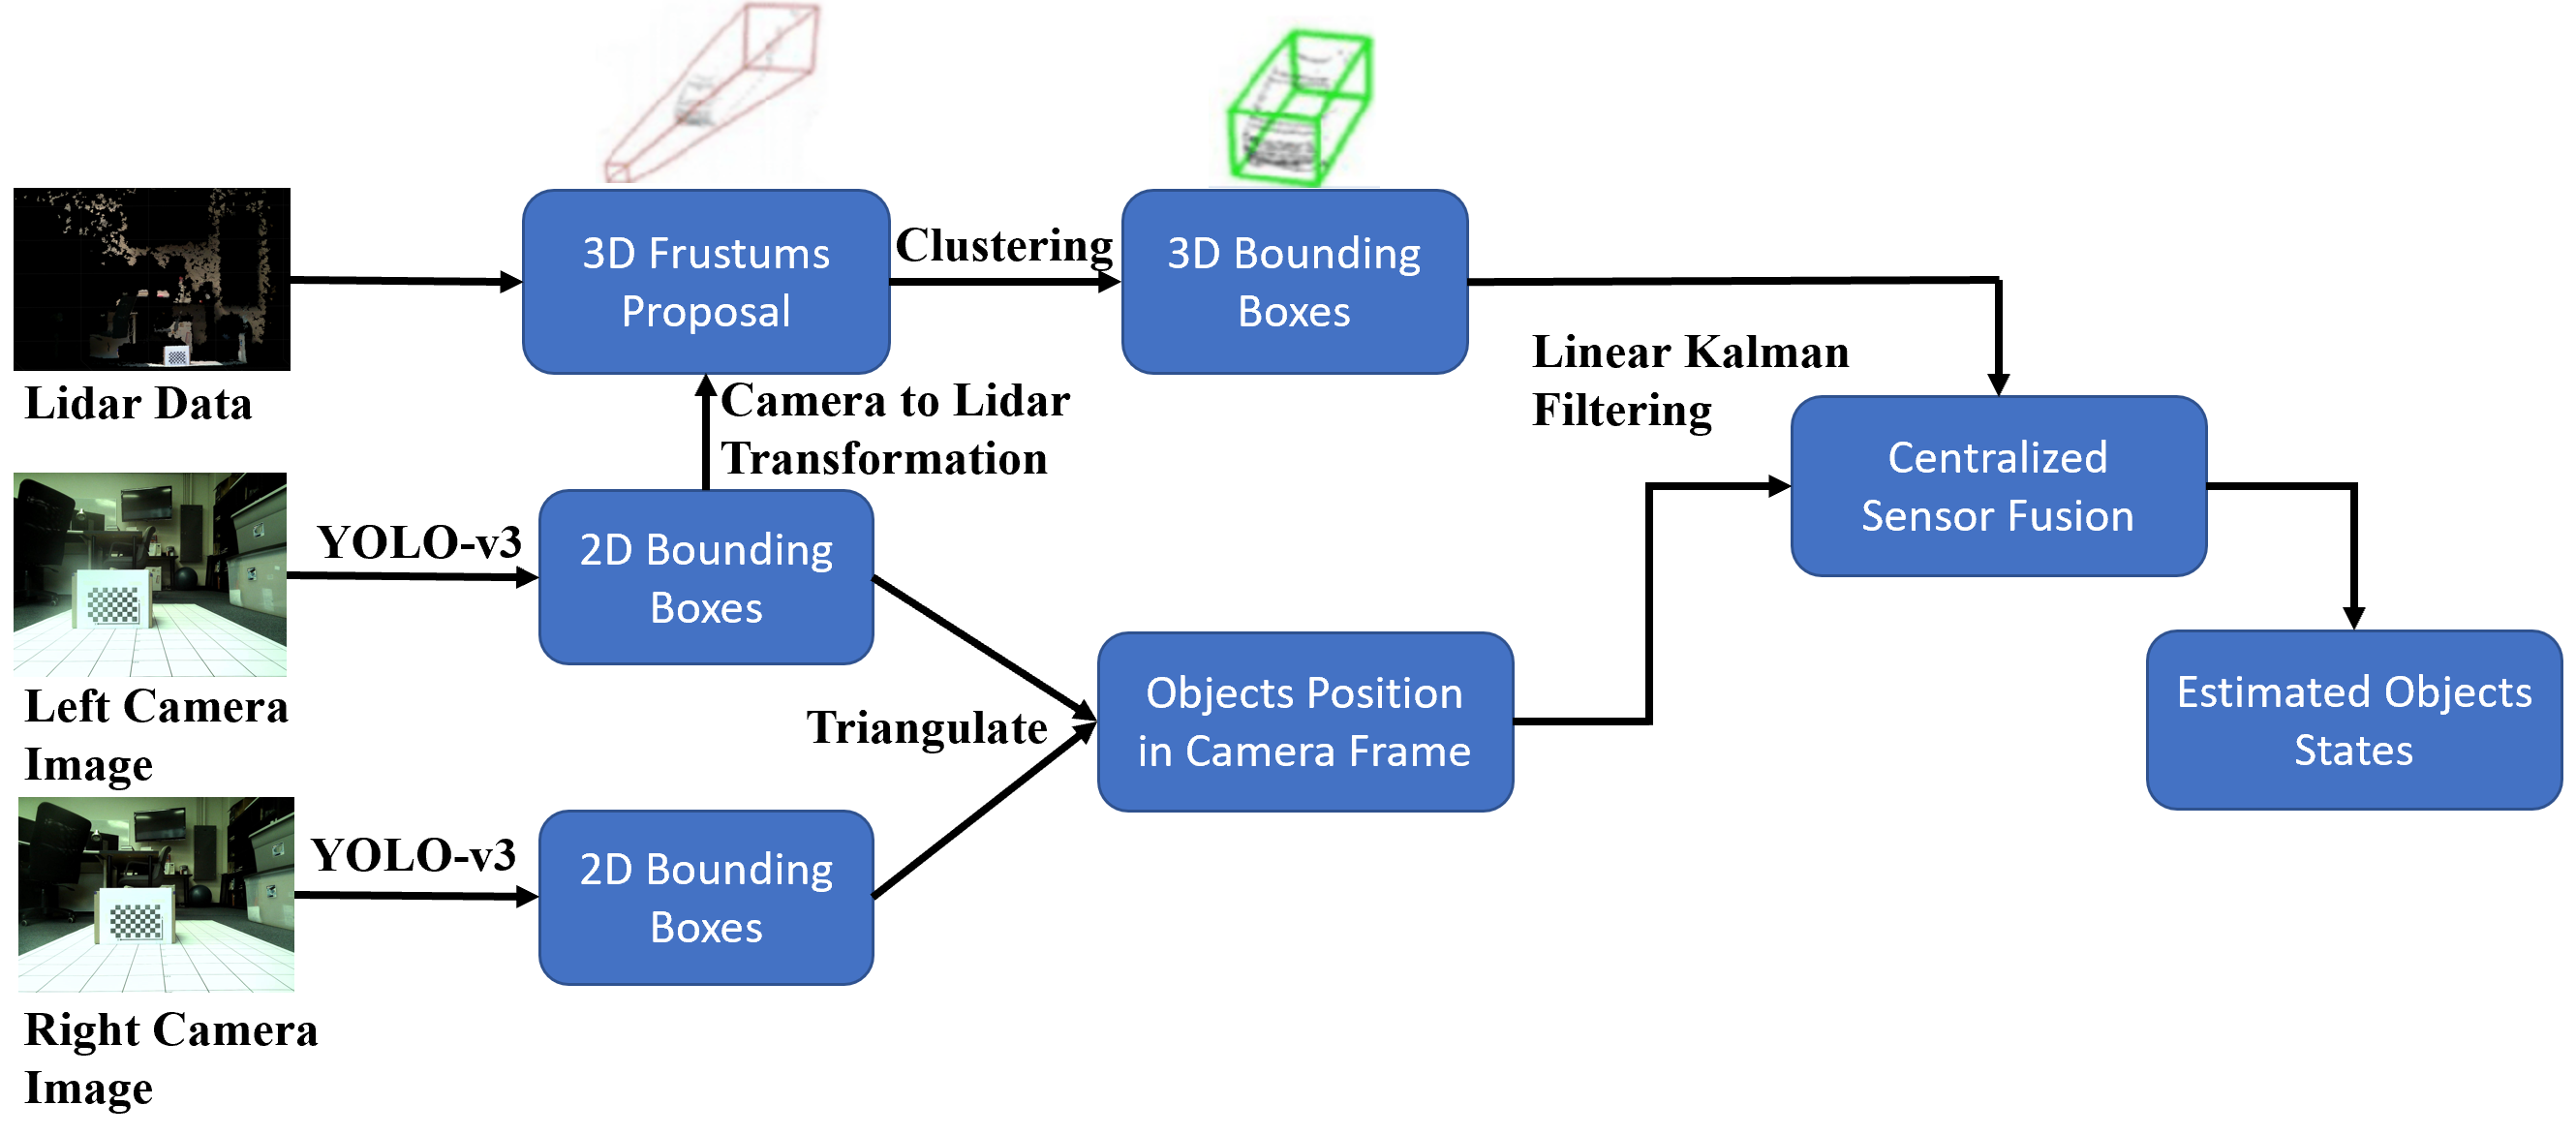
\includegraphics[scale=0.18]{Images/Datapipeline.png}
    \caption{Data Pipeline of Research Work}
    \label{Datapipeline}
\end{figure}

\section{Contributions} 
The list of contributions in this thesis are listed below. 

\begin{itemize}
    \item Performed a transfer learning on pre-trained Convolutional neural network YOLOv3 by using Stochastic Gradient Descent Method (SGDM) for object detection and classification. 
    \item Iteratively performed supervised learning by tuning hyper-parameters such as L2 regularization parameter, Learning rate, mini-batch size, numbers of epochs, and learning momentum to improve the performance of the detector.
    \item Accomplished evaluation of the trained model in real-time using the pre-labeled test dataset.
    \item Perform an intrinsic and extrinsic calibration of optical sensors stereo camera and LiDAR to find their standard measurement errors,  co-variance, and euclidean transformation between two sensor frames. 
    \item Implemented a sensor fusion framework for constant acceleration motion model by using linear Kalman filter in a simulation environment. 
    \item Implemented a sensor fusion on hardware for real-time application after successful testing in a simulated environment.
\end{itemize}



